\documentclass[aps,pre,twocolumn,showpacs,amsmath,amssymb]{revtex4-1}

\usepackage{graphicx}
\usepackage{color}
\usepackage{float}

\usepackage[portuguese]{babel}
\usepackage[utf8]{inputenc}
\usepackage[T1]{fontenc}

\usepackage[export]{adjustbox}

\hfuzz 1pt
\vfuzz 1pt

\setlength{\parskip}{\baselineskip}

\begin{document}

\title{Exercício 8: Análise de Dados (parte I)}

\author{Ernesto González nº(52857) , Rodrigo Januário nº(53087), André Nunes nº(52868)}

\begin{abstract}
Análise de resultados das eleições americanas de 2008 e 2016. Estudo de séries temporais de medição de número de Wolf, associado às manchas solares e correlação com a temperatura média global mensal. Análise da ocorrência de terramotos em Lisboa.
\end{abstract}

\maketitle
% \section{Introdução}
% No primeiro exercício realizou-se uma analise estatística dos dados relativos as eleições de 2008 nos Estados Unidos. Começando pelo calculo da media, mediana e variância dos votos por estado para os dois candidatos, Barack Hussein Obama II e John Sidney McCain III. Seguida pela construção de dois histogramas que refletem a diferença de votos entre ambos os candidatos. O principal objetivo do estudo foi compreender quais os principais efeitos que influenciam o resultado das eleições, analisando a distribuição de votos e a margem de vitória de um candidato.
\section{Análise de dados eleitorais}
\subsection{Eleições presidenciais americanas 2008}
Usando a biblioteca Statistics do python aplicamos as funções: \verb mean  para calcular a media, \verb median  para calcular a mediana e \verb pvariance  para calcular a variância. Obtendo os seguintes valores para cada candidato: \\
\begin{table}[h!]
\caption{Média, mediana e variância de votos por condado, para cada candidato, nas eleições presidenciais americanas de 2008.}
\begin{tabular}{|l|c|c|c|c|}
\hline
 & Barack Obama & John McCain \\ \hline
Média & 21407.07 & 18726.90 \\ \hline
Mediana & 4473 & 6244 \\ \hline
Variância & 5273664087.51 & 1848072555.97 \\ \hline
\end{tabular}
\end{table}
\vspace{1 cm}
De seguida, construíram-se dois histogramas, o da Figura 1 (a) onde se contabilizaram todos os municípios e o da Figura 1 (b) onde se consideraram apenas os municípios com mais de 20 000 eleitores. Para ambos os gráficos criou-se uma relação entre $F_v = v_O-v_M$ e $N_c$, onde $F_v$ representa a diferença entre os votos do Obama $v_O$ e os votos do McCain $v_M$, e $N_c$ a frequência absoluta, ou seja, o número de vezes que observamos diferença relativa (dada por $F_v/n$, em que $n$ são o numero total de eleitores por município) dentro do intervalo a que corresponde cada barra do histograma. Para fazer os histogramas realizou-se o seguinte processo: para cada município, se o número de votos de Obama fosse superior aos de McCain, a diferença relativa era um valor positivo e, portanto, $F_v$ era guardada numa lista de valores positivos, indicando uma maior probabilidade do Obama sair vencedor. Caso contrário, a diferença relativa $F_v$ era guardada numa lista de diferenças relativas negativas, aumentando as hipóteses de McCain ganhar as eleições.
% \begin{figure}[h!]
%     \centering
%     \includegraphics[width = 8.8cm]{histograma1.PNG}
%     \caption{Histograma de todos os municípios, onde $v_O - v_M \in[-1.0; 1.0]$ representa a diferença na fração de votos e $N_c \in [0; 500]$ é a frequência absoluta.}
% \end{figure}
% \begin{figure}[hbt!]
%     \centering
%     \includegraphics[width = 8.8cm]{histograma2.PNG}
%     \caption{Histograma de municípios com mais de 20 mil eleitores, onde $v_O - v_M \in [-1.0; 1.0]$ representa a diferença na fração de votos e $N_c \in [0; 200]$ é a frequência absoluta.}
% \end{figure}

\begin{figure}[hbt!]
    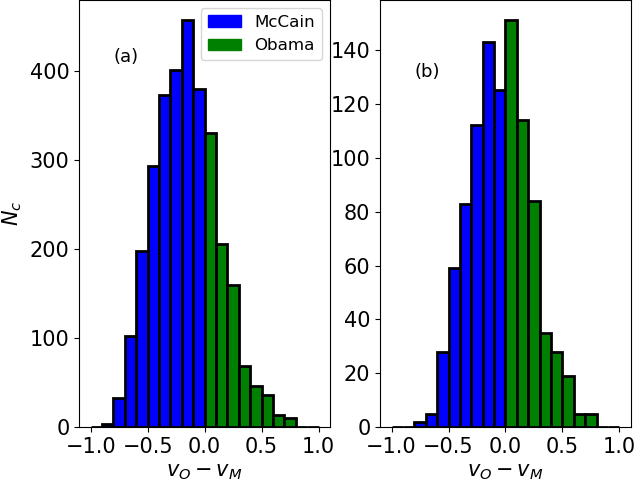
\includegraphics[scale=0.53,left]{obamamccaincounties.png}
    \caption{Histogramas da diferença relativa de votos por condado, $v_O-v_M$, para as eleições presidenciais americanas de $2008$, considerando todos os condados no histograma (a) e apenas os condados com mais de $20000$ no histograma (b).}
\end{figure}

Pela análise da Figura 1 (a), concluímos que o histograma segue uma distribuição Gaussiana com valor médio de $-0.3$, resultado de uma maior frequência de municípios em que McCain obteve mais votos que o Obama, o que deveria refletir uma clara vitoria por parte de McCain. No entanto, ao eliminar os municípios com menos de $20 000$ eleitores, Figura 1 (b), as diferenças relativas que ultrapassam os $0.5$ são desprezáveis e deixamos de ter uma distribuição aproximadamente Gaussiana. Levando a uma vitoria por parte de Barack Obama por uma pequena margem, comprovando a teoria dada no enunciado do trabalho.
% Na figura 4 verificam-se duas colunas a mais do que a do histograma do artigo artigo, isto aconteceu devido à escolha do bin ser diferente. Optou-se por escolher o número de bins iguais ao número de colunas de cada histograma. É ainda importante referir que o tamanho do bin tem influência na precisão dos dados representados. Isto é, um bin muito elevado diminui a precisão dos dados, mas um bin muito pequeno pode originar inconsistência dos resultados, uma vez que estes não são analisados numa escala amplificada.

\subsection{Eleições presidenciais americanas 2016}
As eleições presidenciais americanas 2016, na sua fase final, foram concorridas por Hillary Clinton e Donald Trump. Nesta subsecção seguimos o mesmo procedimento seguido nas eleições de 2008.\\
A Tabela II apresenta a média, mediana e variância de votos por condado, para cada candidato.\\
\begin{table}[hbt!]
\caption{Média, mediana e variância de votos por condado, para cada candidato, nas eleições presidenciais americanas de 2016.}
\begin{tabular}{|l|c|c|c|c|}
\hline
 & Hillary Clinton & Donald Trump \\ \hline
Média & 20042.195 & 19635.71 \\ \hline
Mediana & 3155 & 7169 \\ \hline
Variância & 5168264802.05 & 1632003748.04 \\ \hline
\end{tabular}
\end{table}
A Figura 2 apresenta os histogramas das diferenças relativas de votos por condado, $v_C-v_T$, em que $v_C$ são os votos obtidos por Hillary Clinton e $v_T$ os votos obtidos por Donald Trump no condado. Semelhante à subsecção I.A., na Figura  2 (a) foram considerados todos os condados americanos e na Figura 2 (b) apenas condados com mais do que $20000$ votantes.

\begin{figure}[hbt!]
    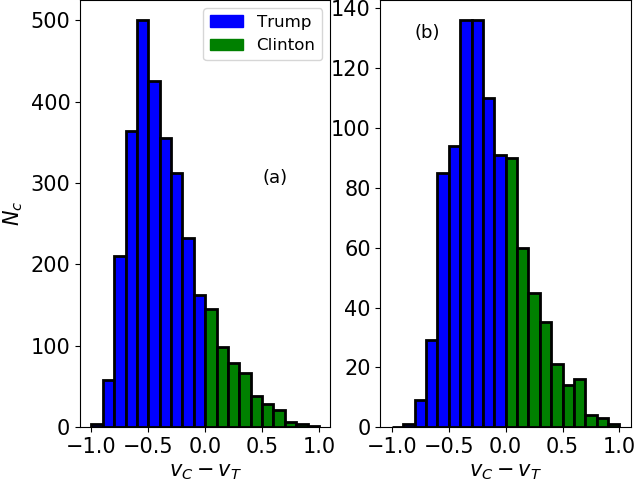
\includegraphics[scale=0.53,left]{clintontrumpcounties.png}
    \caption{Histogramas da diferença relativa de votos por condado, $v_C-v_T$, para as eleições presidenciais americanas de $2016$, considerando todos os condados no histograma (a) e apenas os condados com mais de $20000$ no histograma (b).}
\end{figure}

\section{Evolução das manchas solares}
\subsection{Série temporal da medição do número de Wolf}
Nesta parte do trabalho, pretende-se estudar a evolução das manchas solares, com base em dados recolhidos mês a mês entre janeiro de 1749 e dezembro de 1983. As manchas solares são medidas pelo número de Wolf, $W$, dado por
\begin{equation}
    W = k(10g + f),
\end{equation}
onde $k$ é um fator da escala, $f$ o número de manchas e $g$ o número de grupos. Para tal, começa-se por traçar o gráfico das manchas solares em Wolf em função do mês em que foi medido (Figura 3).

\begin{figure}[hbt!]
    \centering
    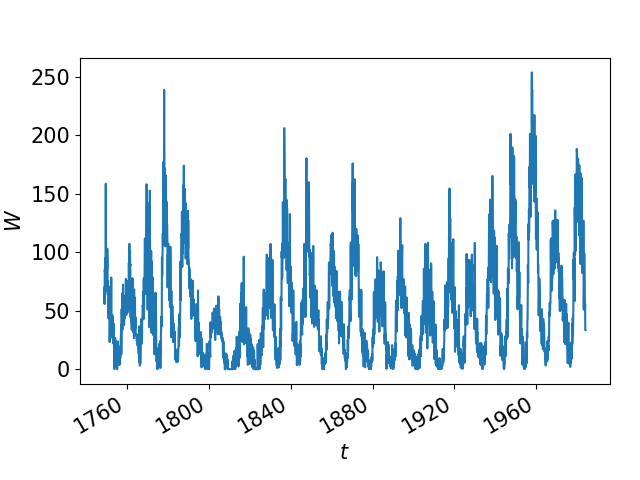
\includegraphics[width=\columnwidth]{temporalseries.png}
    \caption{Gráfico do número de Wolf, $W$, medido em cada mês, para meses entre janeiro de 1749 e dezembro de 1983.}
\end{figure}

Como podemos observar, a curva aparenta ter uma certa periodicidade. No entanto, devido à natureza dos dados, estes apresentam \textit{ruído}, que pode estar associado à incerteza de medição ou por flutuações características. Assim, para podermos encontrar a periodicidade, precisamos de traçar o gráfico da autocorrelação, isto é, como é que a série de dados se relaciona consigo mesmo no tempo. Para tal, aplicámos a equação
\begin{equation}
    r_k = \frac{\frac{1}{N-k}\sum_{t=1}^{N-k}(y_t - \bar{y})(y_{y+k} - \bar{y})}{\frac{1}{N}\sum_{t=1}^{N}(y_t - \bar{y})^2}
\end{equation}
em todos os valores de $t$, iterando sobre $k$, para encontrarmos o período que melhor se ajusta aos dados. Obteve-se então o gráfico da Figura 4.\\

\begin{figure}[hbt!]
    \centering
    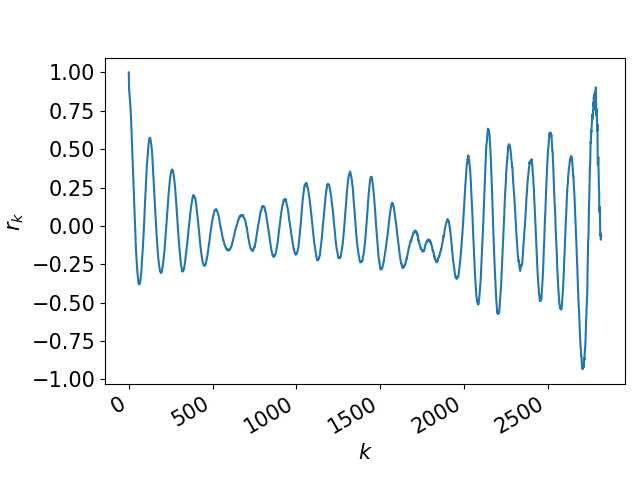
\includegraphics[width=\columnwidth]{autocorrelation.png}
    \caption{Gráfico da função autocorrelação, $r_k$, para a medição mensal do número de Wolf, medido entre janeiro de 1749 e dezembro de 1983, e intervalos de tempo $k$ de até 2800 meses.}
\end{figure}

Da Figura 4, vemos que a medição mensal do número de Wolf tem dependência sazonal: o gráfico da autocorrelação apresenta máximos e mínimos locais de forma periódica. Significa que o número de Wolf $W(t)$ depende do número de Wolf $W(t-T)$ para o período $T$ das \textit{seasons} de máximos e mínimos. Esse período $T$ pode ser obtido medindo a diferença de tempo entre os dois primeiros mínimos locais no gráfico da autocorrelação. Desta forma, obtemos $T=128$.\\
De forma a excluir a sazonalidade do número de Wolf, estudamos o comportamento de $W(t)-W(t-T).$ Na Figura X encontra-se o gráfico desta função.

\begin{figure}[hbt!]
    \centering
    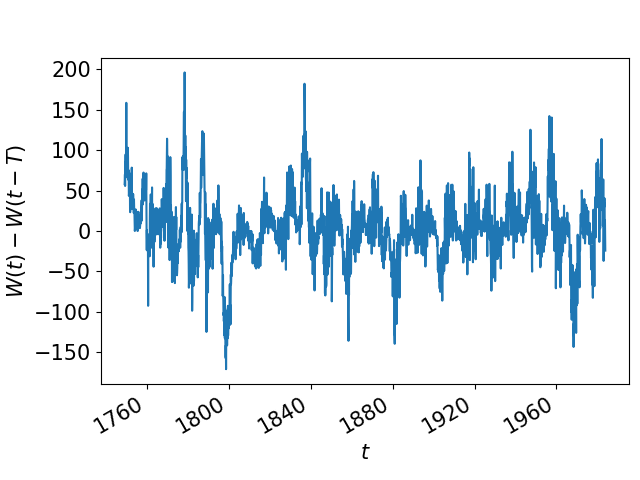
\includegraphics[width=\columnwidth]{seasonaldifference.png}
    \caption{Série temporal da medição mensal do número de Wolf, $W$, entre janeiro de 1749 e dezembro de 1983, aplicadas diferenças sazonais, $W(t)-W(t-T)$, para um período $T=128$ meses.}
\end{figure}

\subsection{Temperatura média global e número de Wolf}
Considere-se a variação da temperatura média global. A Figura 6 apresenta a série temporal da variação da temperatura média global mensal à superfície.\\

\begin{figure}[hbt!]
    \centering
    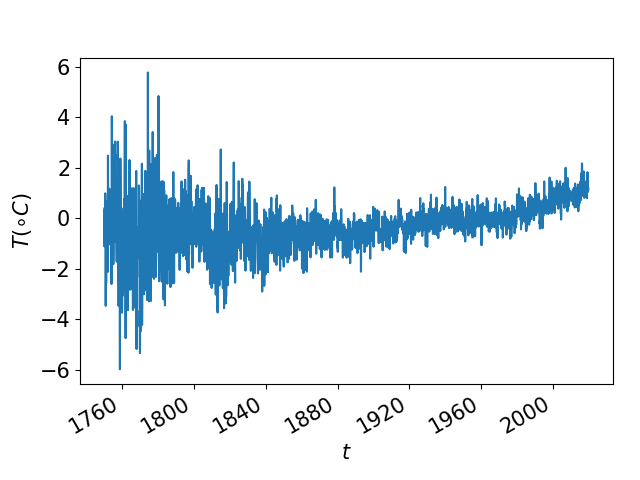
\includegraphics[width=\columnwidth]{averageglobaltemperature.png}
    \caption{Série temporal da temperatura média global mensal à superfície, $T$, em graus centígrados, entre janeiro de 1951 e setembro de 2019.}
\end{figure}

Consideremos a trajetória $W(T(t))$ da medição mensal do número de Wolf, $W(t)$ e da temperatura média global mensal à superfície, $T(t)$. Encontra-se na Figura X os pontos desta trajetória desde janeiro de 1750 até dezembro de 1983, com exceção de dezembro de 1751.\\

\begin{figure}[hbt!]
    \centering
    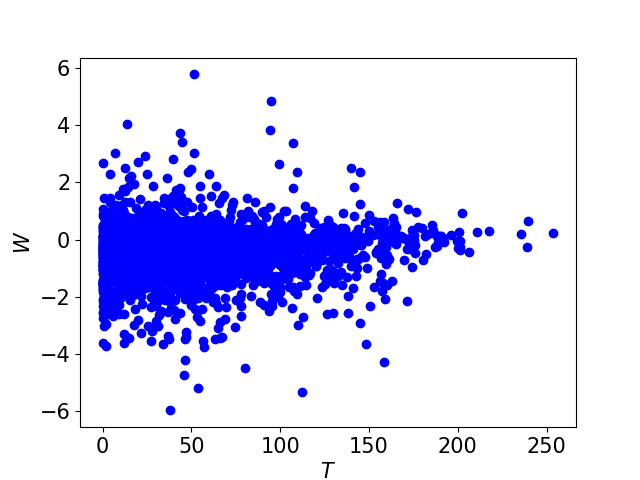
\includegraphics[width=\columnwidth]{wolfandtemperature.png}
    \caption{Gráfico dos pontos da trajetória da medição mensal do número de Wolf, $W$, em função da temperatura média global mensal superficial, $T$, em centígrados.}
\end{figure}
Da análise da Figura 7, vê-se que os pontos da trajetória da medição mensal do número de Wolf em função da temperatura média global mensal superficial, $W(T)$, estão concentrados num triângulo isósceles com base em $T=0$ e e altura ao longo de $W=0$, logo há algum tipo de correlação entre $W$ e $T$ medidos num determinado mês.
O coeficiente de correlação de Pearson entre $W$ e $T$ é
\begin{equation}
    R_P=\frac{cov(W,T)}{\sigma_W \sigma_T}=0.06667595918293301.
\end{equation}
O coeficiente de correlação de Pearson, $R_P$, neste caso é bastante baixo, não refletindo a correlação observada na Figura 7. Deve-se a que este coeficiente apenas considera correlação linear entre as duas variáveis, que não é o nosso caso.
\end{document}
